\documentclass[11pt,a4paper]{article}
\usepackage{tabularx}
\usepackage{ltablex}
\usepackage{graphicx}
\usepackage[cache=false]{minted}
\setminted[erlang]{
frame=lines,
framesep=2mm,
baselinestretch=1.1,
fontsize=\footnotesize,
linenos,
breaklines}
\setminted[haskell]{
frame=lines,
framesep=2mm,
baselinestretch=1.1,
fontsize=\footnotesize,
linenos,
breaklines}
\setminted[bnf]{
frame=lines,
framesep=2mm,
baselinestretch=1.1,
fontsize=\footnotesize,
linenos,
breaklines}
\usemintedstyle{friendly}
% Add Subtitle
\usepackage{titling}
\newcommand{\subtitle}[1]{%
  \posttitle{%
    \par\end{center}
    \begin{center}\large#1\end{center}
    \vskip0.5em}%
}

\begin{document}

\title{Advanced Programming Exam 2018}

\author{Exam Number: 95, Username: zlp432}
\date{\today}
	
\maketitle
\tableofcontents

\section{Utility functions}
The Code for this task is attached in the appendix \ref{appendix:question1-1}.

\subsection{Version}
The Implementation of Version is relatively straight forward and throughly tested by unit tests, which include the examples from the exam text.
I did ended up with a not working implementation before, so I ended up reimplementing the function which is now working as it should.

\subsection{Merge}
Merge is implemented as described in the exam text and tested with many different examples in the unit tests, which all run through.
I had some problems with matching the constraints together, since I kind of lost overview of the function.
Especially ending up when merging only with same package and the different ones (not matching) where not added to the resulting list but in the end just forgot to append the rest to the result.

\subsection{Assessment}
The Utility functions seems to work as intended, as least I was able to reuse them in the parser, and thanks to lots of unit tests to both functions I do believe they work as they should.

\section{Parsing appm databases}
The Code for this task is attached in the appendix \ref{appendix:question1-2}.
\subsection{Choice of parser library}
I implemented the Parser for appm in parsec, mostly out of this reason:
\begin{itemize}
	\item Better Error handling compared to ReadP
	\item I do have more experience with Parsec then ReadP (Assignments)
\end{itemize}

I did end up using \textbf{try} quite a lot, which wasn't my intention at all but with the presented Grammar I haven't found a better solution and overall the parser works more or less.

\subsection{Transforming Grammar}
I decided to make a more strict choice about the Clauses, by parsing them in a fixed ordering (name first etc.), I didn't find much of a better solution for that grammar (making it more dynamic and of course also reduced the complexity of the parser).
The existing grammar has some ambiguities (could have had many names, description etc.), for that case I transformed the Grammar a little so that it matches more to my idea.
So that Name comes first (at least once) and then one after the other follows or is set to empty.
Technically Version, Description etc. could show up more then once but those cases are not handled in the Parser
\begin{minted}{bnf}
Database ::= \epsilon
			| Package Database
Package ::= 'package' '{' Clauses '}'
Clauses ::= \epsilon
			| Clause
			| Clauses ';' Clauses
Clause ::= 'name' PName Version
Version ::= \epsilon
			| 'version' Version 
			| Description
Description ::= \epsilon
				| 'description' String 
				| Constraints
Constraints ::= \epsilon	
			|'requires' PList
			|'conflicts' PList									

PList ::= 	PItem
		| PList ‘,’ PItem
PItem ::= PName
		| PName ‘>=’ Version 
		| PName ‘<’ Version
Version ::= (see Text)
PName ::= (see Text)
String ::=(see Text)		
\end{minted}

Since I don't know what exactly will follow after a Name I use try in all the following calls of parsing one of the clauses (Version etc.), this way I can skip one or the other except for the name.

\subsection{Assessment}
\subsubsection{Scope of Test Cases}
I did quite a few unit tests for the parser (including failing ones), since not everything ended up to be working or there was just not enough time left to fix all the bugs which showed up.
Overall I tried to test as many cases as possible, which I think I succeeded in because I did find some bugs throughout the development process thanks to the testing.

\subsubsection{Correctness}
The Solution is far from perfect, but it was able to parse the example intro to the preferred outcome.
There are a few bugs on of which is the ordering of requires and conflicts, so in case I want to parse \textbf{requires bar >= 3, bar < 2}, this would end in an error since the case of having the greater then version in the first place won't work all the other cases work.
Also adding a comment \textbf{--comment} after the end of the last package doesn't work.
Beside those bugs, there are of course also other ways to get the parser to fail.
For example only by changing the ordering of clauses and lots of other things.
So for a well-formed package (ordering is right, only one clause of name, version etc.) the parser works, in lots of other cases the parser might fail.

\subsubsection{Code Quality}
I do believe the code is more or less easy to read, I tried to put the things together which belong together which should help understanding it easier.
But nonetheless I'm not satisfied with how many tries I needed to solve the task and also the left over bugs which I wasn't able to fix until the end of the exam.
On the other hand I'm also quite happy that was I able to put some more functionality into the parser as I thought beforehand I would do, like the string parsing, caseString (keywords can have any case) etc.

\section{Solving appm constraints}
skipped since time ran out
\section{Testing appm properties}
skipped since time ran out

\section{The district module}
The code for this task can be found in Appendix \ref{appendix:question2-1}
\subsection{Implementation}
The earls of Ravnica can be seen as a state machine for which I chose to use gen\_statem.
The following states exist:
\begin{itemize}
	\item \textbf{Under Configuration} The initial state of every district, connections can be created, the description called and so on
	\item \textbf{Under Activation} As soon as someone calls \textbf{activate}, the server will switch to this intermediate state until all it's neighbors (connections) are active
	\item \textbf{Active} Server is active and Players can enter, take\_actions and so on
	\item \textbf{Shutting down} Intermediate state before being fully shut down, since all neighbors also have to be shutdown
\end{itemize}

So a District Server can go through following states:

\begin{figure}[!htb]
	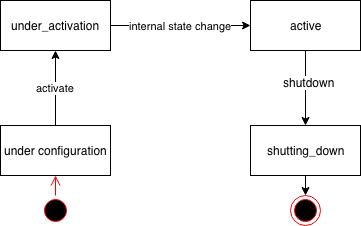
\includegraphics{images/ravnica}
	\caption{Simple State machine diagramm}
\end{figure}

\subsection{Data Structure}
The Data structure I used to implement Ravnica consists of a map with following entries:
\begin{itemize}
	\item \textbf{description} Saves the description which gets saved when starting a server
	\item \textbf{connections} Map for Handling the connections from one District to an other
	\item \textbf{creatures} Map for handling all the entered/active creatures on a Server
	\item \textbf{trigger} Set a trigger for a district, which gets called when a creature is leaving or entering a district
\end{itemize}

\subsection{States}
In the end I ended up with the described states in which a district can be in.
Each state only accepts a number of messages (for example, enter is not allowed in some states and so on),
all unhandled Messages (Technically can send any kind of message when the PID is known) will be ignored but the server will be keep going.
A maybe new thing I did for the exam is using a internal next\_state state change, to be able to switch to those intermediate states when needed.

\subsection{Communication}
All communication between the districts and to the district is synchronous, this mostly for actually know what kind of state the other neighbors have and I do want to know when every neighbors shutting down or that there is an issue with that.

\subsection{Cycles}
My solution can handle cycles, but it's a very basic solution which definitely won't hold for all kind of cycles.
Even though I did a test on cycles (self cycles and cycles with neighbors), which was succesfully.
In the end my Solution is about checking the \textbf{From} and \textbf{To} PID in case they are the same don't end the message further otherwise we end up in a never ending loop.
Same for when the PID matches with the own PID of the server (self cycles), \textbf{self()} and \textbf{To} are the same.
\begin{figure}[!htb]
\center
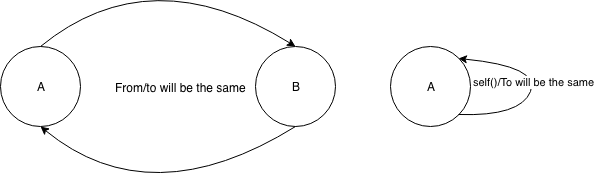
\includegraphics[width=\textwidth]{images/cycles}
	\caption{Showcasing the cycles}
\end{figure}

So this very basic solution will fail for bigger cycles, because here the shutdown or activate message won't be sent from the original district (on which the activate or shutdown got called), so can't be checked according to the \textbf{To} and \textbf{From} PID anymore.

\begin{figure}[!htb]
	\center
	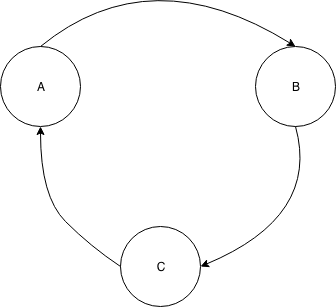
\includegraphics[width=0.5\textwidth]{images/fail_cycle}
	\caption{Example of a failing cycle}
\end{figure}


\subsection{Triggers}
My Solution does support triggers and according to my tests they seem to work.
Also my solution tries to check if a Trigger is well behaved by running it in a different process on which I can set a timeout of 2 seconds, so the server won't break down when a not well behaved trigger runs.
I do check that the Trigger needs to have 3 parameters, so technically any function can be passed with 3 parameters but only if the trigger return the right format which is: \mint{erlang}|{Creature,Creatures}|




\subsection{Assessament}
\subsubsection{Scope of Test Cases}
I did lot of Test cases with \textbf{eunit} which should showcase how much my solution is able to do.
So from Cycles to every call possible (at least in the easiest way), since I don't tested the responses in intermediate states and lots of other things which are not very easy to test just like that.
\subsubsection{Correctness}
According to my tests I do believe I have a somewhat correct solution, even though the nasty cycles are not in total solved/removed.
Otherwise I'm quite confident in my solution and the correctness of it, even though there are probably lots of more nasty test cases I wasn't able to think of in the shot period of time I had.
\subsubsection{Code Quality}
The code quality is somewhat mediocre, since there is lots of repetition and duplicated code which could be removed/improved but out of the time constraints refactoring wasn't my top priority. Therefore the overall code is ok but not really great, at least all helper functions are grouped together, and the states are ordered by how the server will go through them from top to bottom.
\section{QuickCheck district}
The code for this task can be found in Appendix \ref{appendix:tests}
\subsection{Territory Generator}
I did write a Generator for \textbf{territory/0} but I wasn't able to write the Properties for activate and take\_action, since the time ran out.
So I only started on this task but wasn't able to finish it totally.

\appendix
\section{Code Listing}
\subsection{Question 1.1: handin/appm/src/Utils.hs}
\label{appendix:question1-1}
\inputminted{haskell}{handin/appm/src/Utils.hs}
\subsection{Question 1.2: handin/appm/src/ParserImpl.hs}
\label{appendix:question1-2}
\inputminted{haskell}{handin/appm/src/ParserImpl.hs}
\subsection{Question 2.1: handin/ravnica/district.erl}
\inputminted{erlang}{handin/ravnica/district.erl}
\label{appendix:question2-1}

\section{Tests Listing}
\subsection{Question 1.1 and Question 1.2 handin/appm/tests/BB/Main.hs}
\inputminted{haskell}{handin/appm/tests/BB/Main.hs}
\subsection{Question 2.1}
\inputminted{erlang}{handin/ravnica/district_tests.erl}
\subsection{Question 2.2}
\inputminted{erlang}{handin/ravnica/district_qc.erl}
\label{appendix:tests}
\end{document}